\documentclass[a4paper,14pt]{extarticle}

\usepackage[english,russian]{babel}
\usepackage[T2A]{fontenc}
\usepackage[utf8]{inputenc}
\usepackage{ragged2e}
\usepackage[utf8]{inputenc}
\usepackage{hyperref}
\usepackage{minted}
\setmintedinline{frame=lines, framesep=2mm, baselinestretch=1.5, bgcolor=LightGray, breaklines,fontsize=\scriptsize, tabsize=4}
\setminted{frame=lines, framesep=2mm, baselinestretch=1.5, bgcolor=LightGray, breaklines,fontsize=\scriptsize, tabsize=4}
\usepackage{xcolor}
\definecolor{LightGray}{gray}{0.9}
\usepackage{graphicx}
\usepackage[export]{adjustbox}
\usepackage[left=3cm,right=1.5cm,
top=2cm,bottom=2cm,bindingoffset=0cm]{geometry}
\usepackage{fontspec}
\usepackage{ upgreek }
\usepackage[shortlabels]{enumitem}
\usepackage{adjustbox}
\usepackage{multirow}
\usepackage{amsmath}
\usepackage{amssymb}
\usepackage{pifont}
\usepackage{pgfplots}
\usepackage{longtable}
\usepackage{array}
\usepackage{titlesec}
\usepackage{capt-of}
\usepackage{caption} %заголовки плавающих объектов
\usepackage{tocloft}
\usepackage{indentfirst}

\renewcommand{\baselinestretch}{1.5}

\graphicspath{ {./images/} }
\makeatletter
\AddEnumerateCounter{\asbuk}{\russian@alph}{щ}
\makeatother
\setmonofont{Consolas}
\setmainfont{Times New Roman}

\titleformat*{\section}{\centering\bfseries}
\titleformat*{\subsection}{\centering\bfseries}
\titleformat*{\subsubsection}{\centering\bfseries}
\newcommand{\anonsection}[1]{\section*{#1}\addcontentsline{toc}{section}{#1}}

\newcommand\textbox[1]{
	\parbox{.45\textwidth}{#1}
} 

\renewcommand{\cftsecleader}{\cftdotfill{\cftdotsep}} % Add dots between section titles and page numbers
\renewcommand{\cftsecpagefont}{\normalfont} % Set the font for section page numbers

\newcommand{\specialcell}[2][c]{%
	\begin{tabular}[#1]{@{}c@{}}#2\end{tabular}}

\newbox\namebox
\newdimen\signboxdim

\def\signature#1{%
    \setbox\namebox=\hbox{#1}
    \signboxdim=\dimexpr(\wd\namebox+1cm)
    \parbox[t]{\signboxdim}{%
        \centering
%           \mbox{}\leaders\hbox to .4em{\hss.\hss}\hskip\nameboxdim\mbox{}\\   % for dots
            \hrulefill\\    % for a line
            #1
        \par}%
    }
\pretolerance10000

\setlength{\parskip}{0cm}
\setlength{\parindent}{1.25cm}

\begin{document}
\linespread{1.5}
\justifying
\begin{center}
    \small{
        \textbf{МИНИCТЕРCТВО НАУКИ И ВЫCШЕГО ОБРАЗОВАНИЯ РОCCИЙCКОЙ ФЕДЕРАЦИИ}\\
        ФЕДЕРАЛЬНОЕ ГОCУДАРCТВЕННОЕ БЮДЖЕТНОЕ ОБРАЗОВАТЕЛЬНОЕ УЧРЕЖДЕНИЕ\\ВЫCШЕГО ОБРАЗОВАНИЯ \\
        \textbf{«БЕЛГОРОДCКИЙ ГОCУДАРCТВЕННЫЙ ТЕХНОЛОГИЧЕCКИЙ\\УНИВЕРCИТЕТ им. В. Г. ШУХОВА»\\ (БГТУ им. В.Г. Шухова)} \\
        \bigbreak
        
\includegraphics[width=70mm]{log}\\
        ИНСТИТУТ ИНФОРМАЦИОННЫХ ТЕХНОЛОГИЙ И УПРАВЛЯЮЩИХ СИСТЕМ\\}
\end{center}

\vfill
\begin{center}
    \large{
        \textbf{
            КУРСОВОЙ ПРОЕКТ}}\\
    \normalsize{
        по дисциплине: Конструирование программного обеспечения \\
        тема: «Разработка сервиса хранения, версионирования и распространения аудиоданных»}
\end{center}
\vfill
\begin{center}
    Автор работы \signature{\small{(подпись)}} Пахомов Владислав Андреевич ПВ-223\bigbreak
    Руководитель проекта \signature{\small{(подпись)}} Заикин Александр Олегович
\end{center}
\vfill
\begin{center}
    Оценка \signature{}
\end{center}
\vfill\begin{center}
    Белгород 2025 г.
\end{center}
\newpage

\renewcommand{\contentsname}{Оглавление}
\thispagestyle{empty}
\tableofcontents
\newpage

\setlength{\parindent}{1.25cm}

\section{Введение}

Одной из задач при проектировании любого из решений на сегодняшний день является 
организация работы. Это, в том числе, может относиться и к аудиоданным. В данной работе 
будет рассмотрен план развития сервиса для разрешения такой задачи.

Цель курсовой работы заключается в в приобретении практических навыков создания и 
управления программными проектами. Для достижения этой цели необходимо решить следующие
задачи:

\begin{itemize}
    \item Провести анализ предметной области
    \item Декомпозировать и визуализировать задачу
    \item Выбрать наиболее подходящий метод управления для проектирования сервиса
    \item Организовать рабочее пространство управления проекта
    \item Выбрать подходящую систему контроля и мониторинга реализации проекта
    \item Оценить затраты на реализацию и внедрение
    \item Провести анализ внешних и внутренних рисков. Предусмотреть способы их решения
\end{itemize}

\newpage

\section{Анализ предметной области. Создание базовой структуры проекта}
\subsection{Анализ предметной области}
Процесс разработки музыкальных продуктов часто сопряжён с постоянными изменениями 
в составляющих аудиоданных. Было бы полезно иметь возможность быстро проследить, 
как изменялась каждая из версий аудиоданных. Часто возвращение к старым идеям, 
кроме того, может дать толчок для развития в текущей итерации. Также было бы 
полезно иметь возможность распространения определённой версии аудиотрека для 
совместной работы. Возможно, стоит рассмотреть возможность публикации 
полученных результатов в стриминговых сервисах.

Функциональные требования:
\begin{itemize}
\item Безопасность и управление доступом\\
    \begin{itemize}
    \item Аутентификация через Keycloak
    \item Управление портальными ролями (User, Manager, Composer, Admin)
    \end{itemize}
\item Управление сущностями автора
    \begin{itemize}
    \item Возможность создания, редактирования, удаления и просмотра сущности автора
    \end{itemize}
\item Управление сущностями группы
    \begin{itemize}
    \item Возможность создания, редактирования, удаления и просмотра сущности группы
    \item Обеспечение целостности группы
    \end{itemize}
\item Управление сущностями песнями
    \begin{itemize}
    \item Возможность создания, редактирования, удаления версий песен (версионированные данные: название, описание, BPM, тональность, слова, файлы, тэг, публичность)
    \item Переключение между версиями песен
    \item Возможноасть комментирования песен
        \begin{itemize}
        \item Возможность создания, редактирования, удаления и просмотра комментариев, прикреплённых к песне
        \end{itemize}
    \end{itemize}
\item Хранение файлов
    \begin{itemize}
        \item Реализация способа архивации/деархивации аудиофайлов с возможностью потоковой распаковки
    \end{itemize}
\item Управление сущностями плейлистов
    \begin{itemize}
        \item Возможность создания, редактирования, удаления, просмотра плейлистов
        \item Возможность поделиться плейлистом с учётом публичности плейлиста
        \item Возможность создания продвинутых фильтров для подбора конкретной версии песни
    \end{itemize}
\item Воспроивзедение
    \begin{itemize}
        \item Возможность воспроивзедения треков из плейлиста
        \item Воспроизведение нескольких треков
        \item Корректировка аудиопотока с простейшими эффектами, вроде эквалайзера
    \end{itemize}
\item Интеграция со стриминговыми сервисами
\end{itemize}

\subsection{Структура проекта}
Архитектура проекта была выбрана микросервисной. API Gateway будет содержать бизнес-логику
для обработки ролевой модели, сущностей, получения данных от клиента и их валидацией. 
Для стриминга и архивации/деархивации аудиоданных будет использован отдельный сервис.

В качестве стека для первого компонента был выбран стэк из FastAPI, Pydantic, SQLAlchemy, что 
позволяет обеспечить быструю гибкую разработку. 

Второй сервис требует большой скорости и стабильности, поэтому в качестве стека был выбран стек 
язык программирования Rust. 

Инфраструктура может включать в себя сервис авторизации Keycloak. Для развёртывания и масштабирования
необходимо использовать Kubernetes и образы Docker. В качестве базы данных выбран PostgreSQL. 
Для снижения нагрузки на взаимодействие по сети с PostgreSQL можно подключить Redis. 

\section{Декомпозиция и визуализация программного проекта}

Сервис состоит из нескольких микросервисов, выполняющих свою задачу. Архитектуру микросервисов можно 
представить в следующем виде:
\begin{center}
    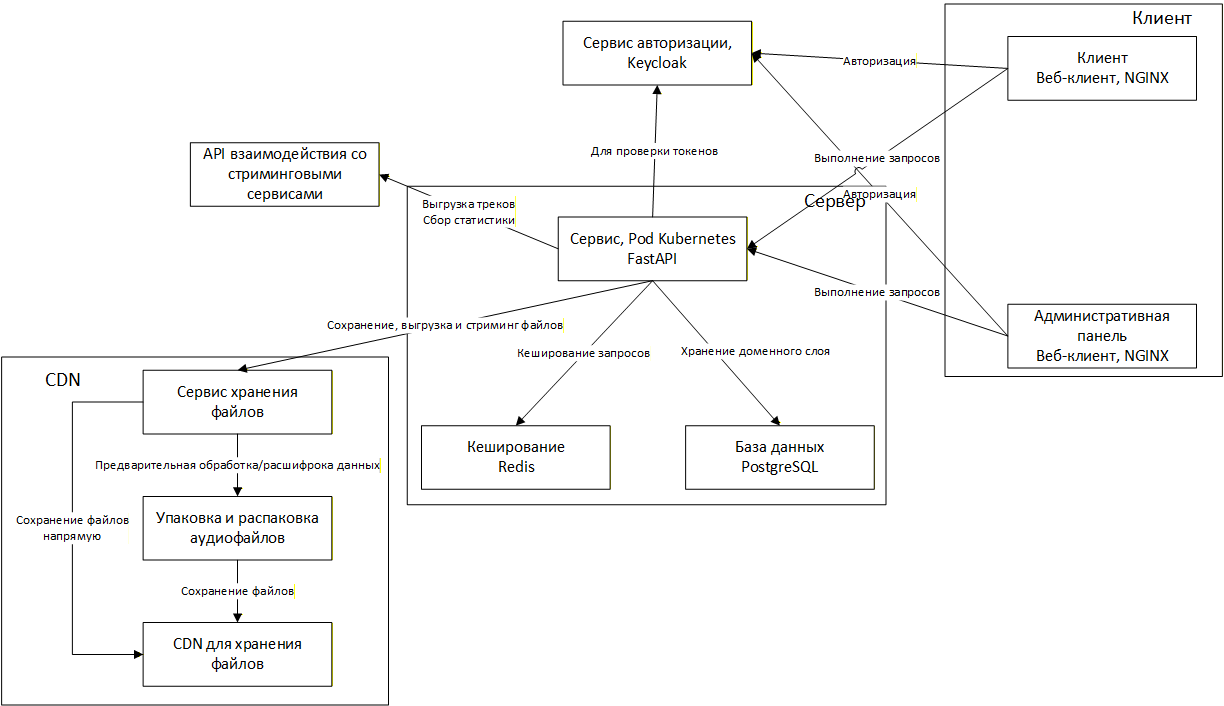
\includegraphics[width=140mm]{vis1}
\end{center}

Структура клиента:
\begin{center}
    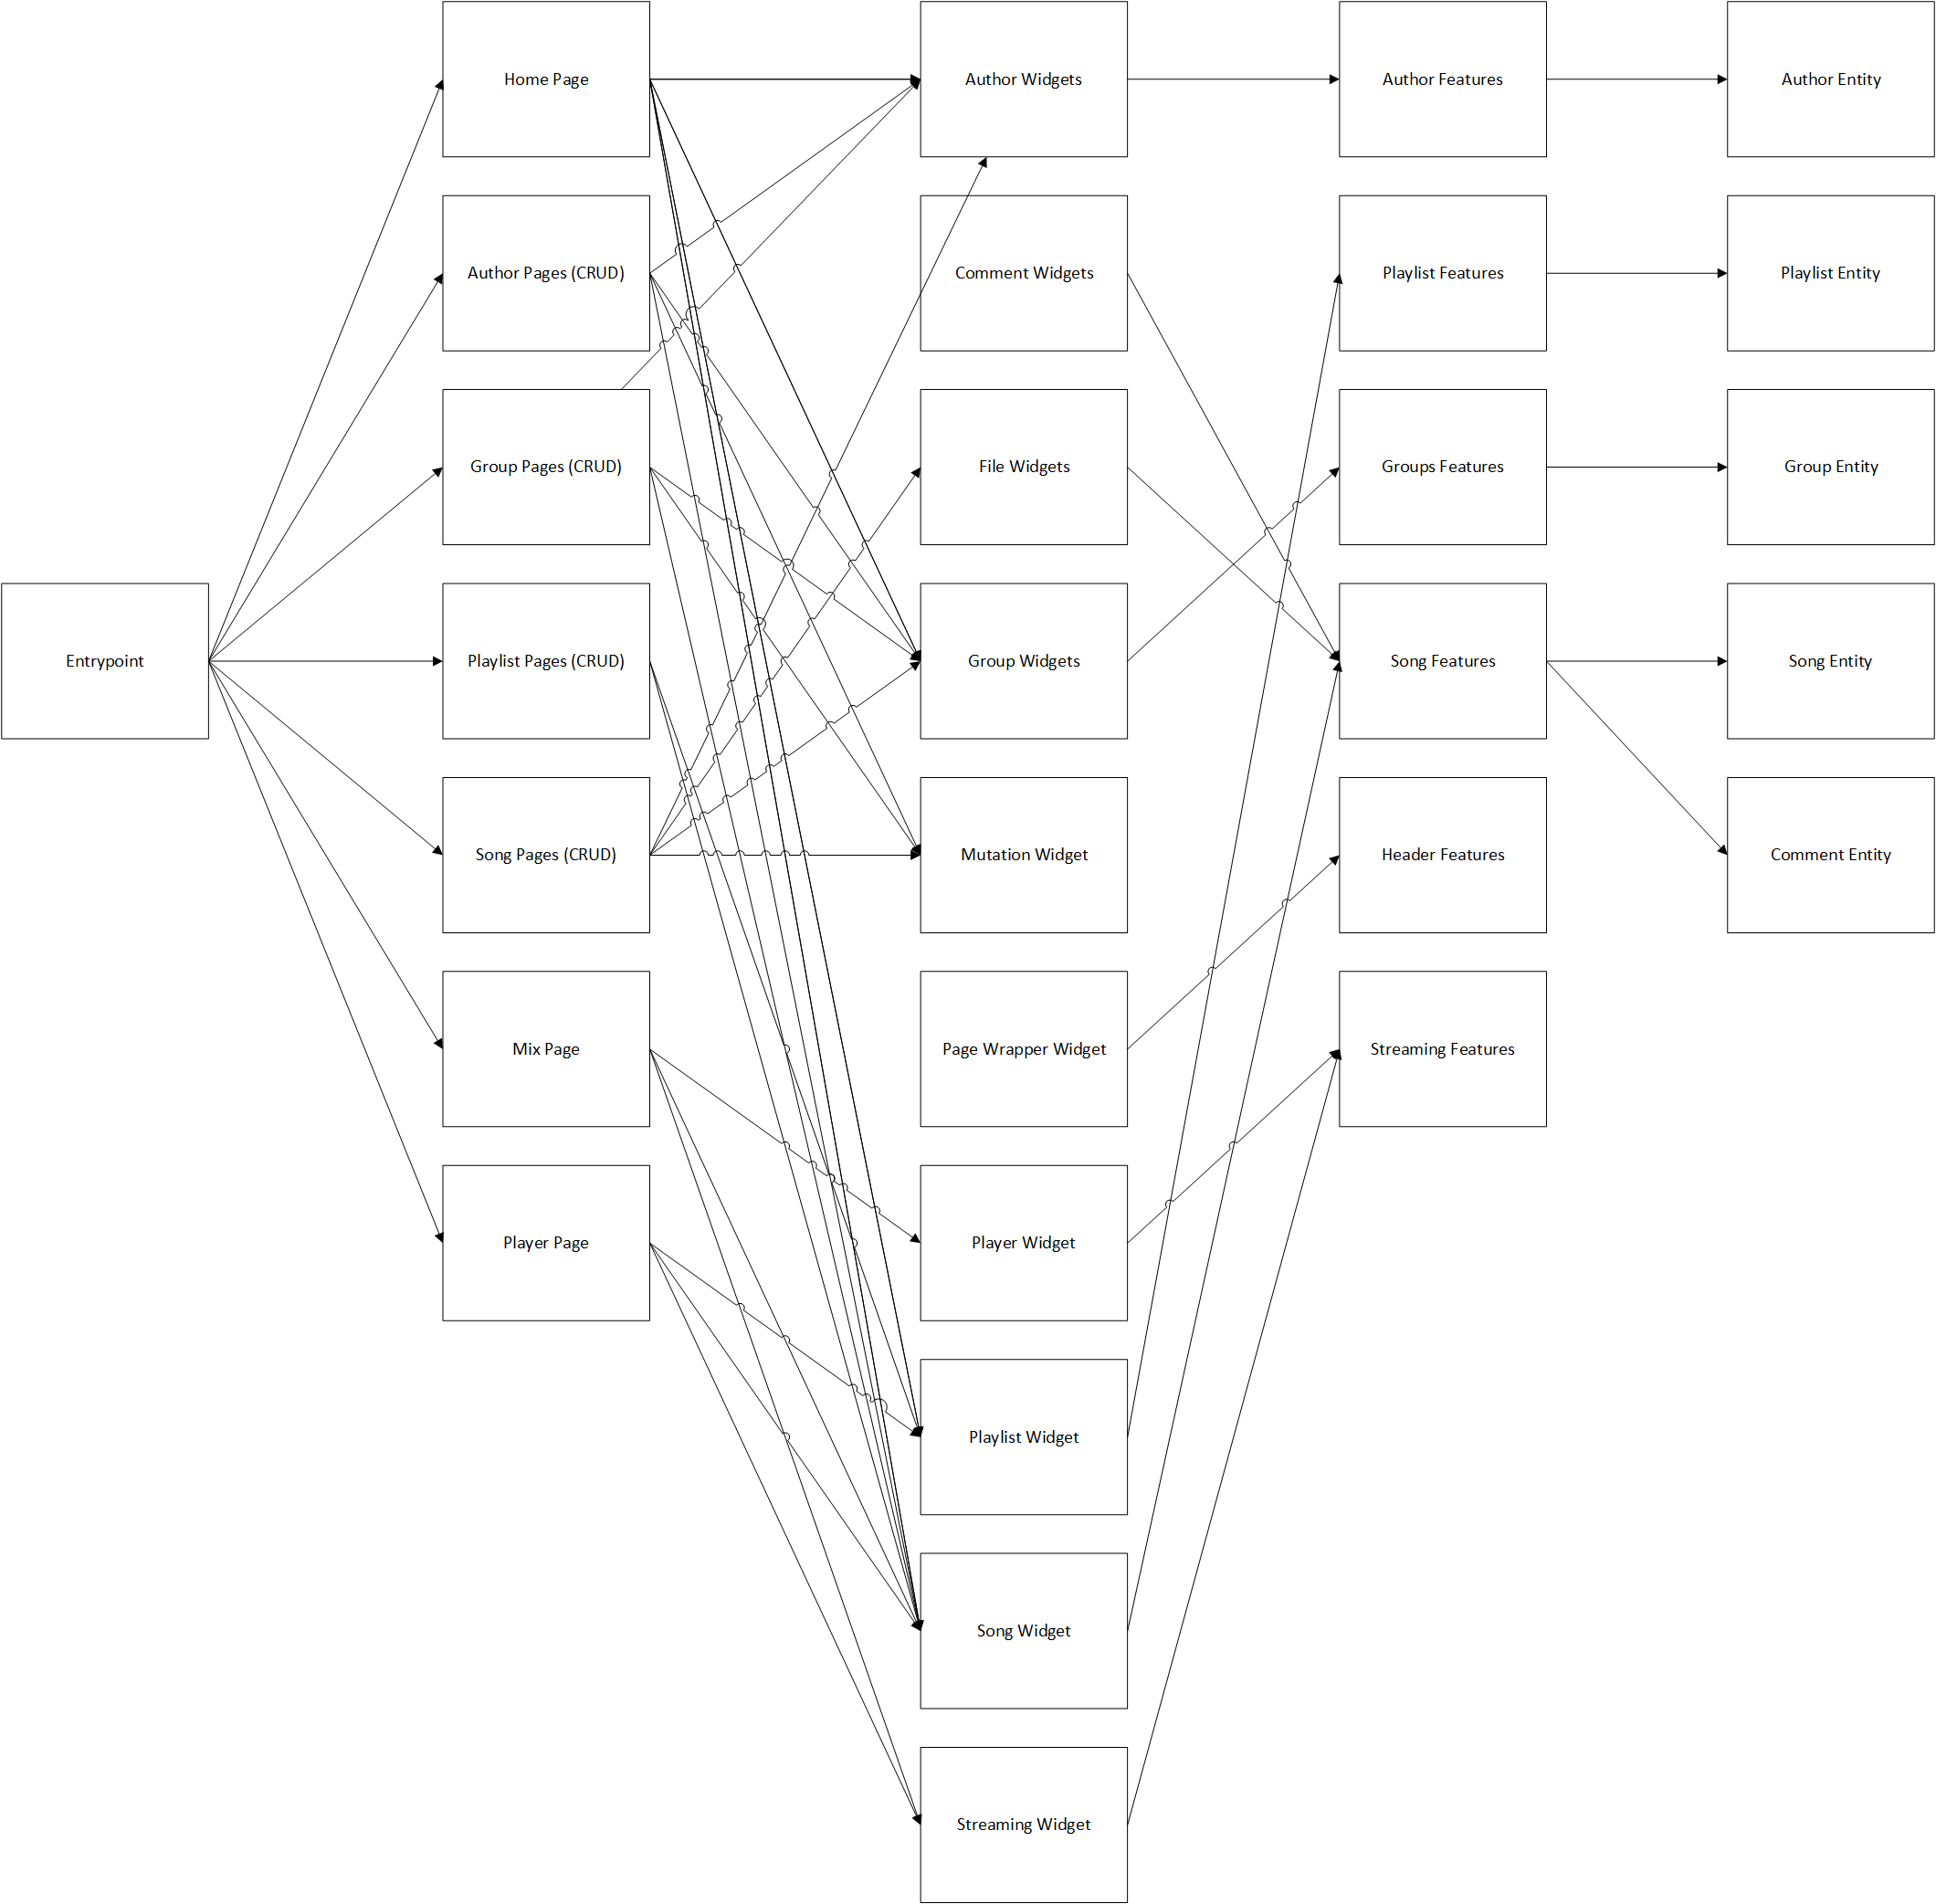
\includegraphics[width=140mm]{arch1}
\end{center}

Структура сервера:
\begin{center}
    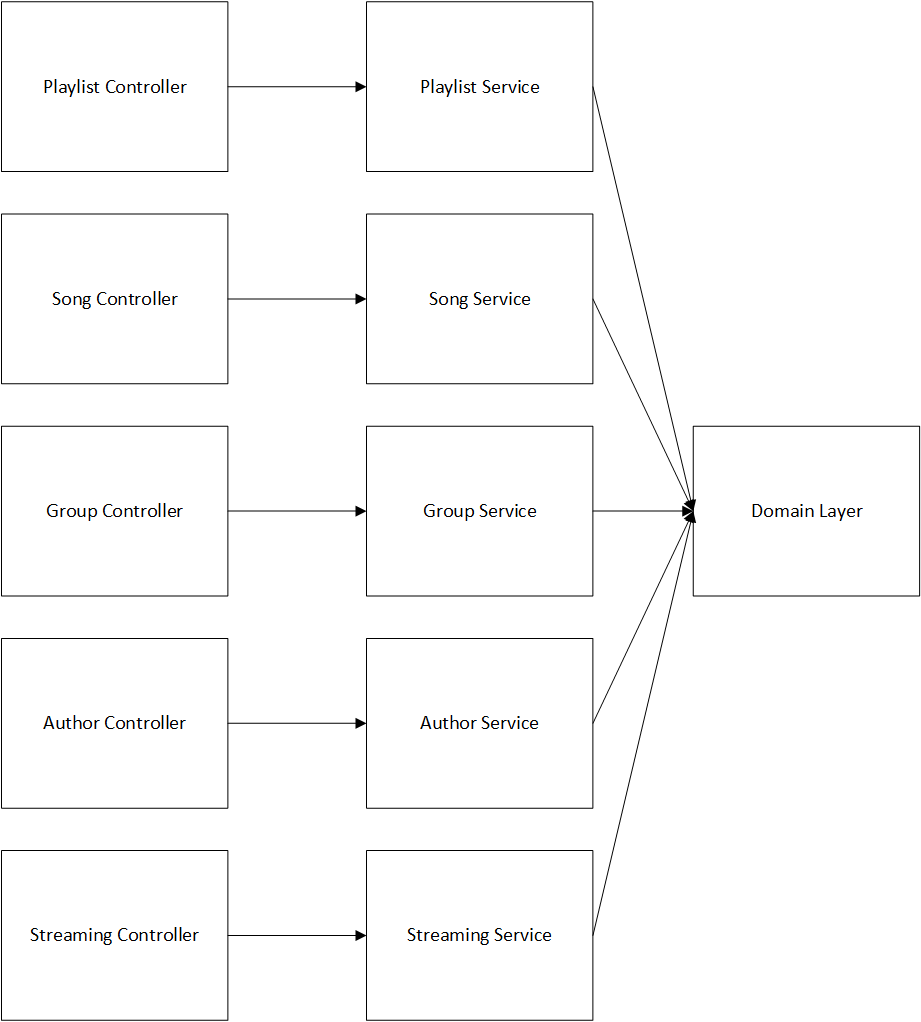
\includegraphics[width=140mm]{arch2}
\end{center}

\section{Методы управления}
\subsection{Выбор и обоснование методологии}
В качестве метода управления был выбран Agile. Данный выбор был обоснован
следующими факторами:
\begin{itemize}
    \item Большая гибкость. Проект является по большей части экспериментальным, 
    множество из предложенных "фичей" проекта могут оказаться ненужными и бесполезными. 
    На первых этапах для проработки концепции можно будет добавить небольшое количество 
    разработчиков и, если проект окажется успешным после опробования, можно будет
    подключить дополнительное количество разработчиков.
    \item Бюджетность. Для проекта не выделяются большие средства на первых
    этапах. Agile позволит подготовить MVP для проверки идеи, и если проект окажется
    успешным, его можно будет развивать дальше.
    \item Отзывчивость. Обратная связь крайне важна для проекта, требования могут
    меняться очень часто. Гибкая методология позволяет адаптироваться к новым
    требованиям. 
\end{itemize}

Методология Agile предполагает разбитие задачи на несколько более мелких подзадач. 
Такие подзадачи позволяют выделить приоритетность и организовать работу. На первых этапах 
необходимо начать разработку с минимально живого сервиса, который будет позволять 
пользователям выстраивать полезные бизнес данные. Задачи подключения к стриминговым
сервисам, оптимизации хранения наименее важны, и их можно отнести к более поздним эпикам. 
Итого получаем:

Эпик 1:
\begin{itemize}
\item Авторизация с помощью Keycloak
\item Версионная модель песен
\end{itemize}
Эпик 2:
\begin{itemize}
\item Группы
\item Авторы
\item Плейлисты
\end{itemize}
Эпик 3:
\begin{itemize}
\item Продвинутый проигрыватель
\end{itemize}
Эпик 4:
\begin{itemize}
\item Оптимизация сервиса хранения данных
\item Интеграция с стриминговыми сервисами
\item Подключение сервиса кеширование, рост сервиса в ширину
\item Дальнейшая оптимизация
\end{itemize}

\section{Организация рабочего пространства управления проектом}
\subsection{Принципы организации рабочего пространства}
Критически важная информация должна быть доступна участникам, храниться в одном месте, 
процессы, особенно критически важные, должны быть автоматизированы,
а также должна быть защищена от потенциальных угроз безопасности. 

\subsection{Инструменты организации рабочего пространства}
В качестве системы контроля версий используется Github с подключением 
собственных раннеров. В проекте у членов команды должна быть своя роль, 
у ролей должны быть настроены разрешения и запреты. Каждый запрос на слияние
должен проходить ревью, а слияние должно проивзодиться ответственным участником команды
(тимлидом). 

Все ключевые данные должны храниться в отдельном волте. Получение ключей при сборке в 
Github Actions должно выполняться через него. 

Код должен иметь единый стиль и форматирование. Настройку форматирования кода передать
DevOps члену команды.

Для хранения полученных образов можно использовать Github Registry и в дальнейшем
self-hosted решение. 

Развёртка приложений и доставка должна происходить автоматически, контейнерезированно. 
Docker контейнеры должны быть развёрнуты в Kubernetes. 
\section{Система контроля и мониторинга реализации проекта}
\subsection{Философия и принципы системы контроля}
Система контроля и мониторинга реализации проекта строится на концепции управления и получения обратной связи
по пунктам, которые измерить важно, а не легко. Контроль осуществляется на операционном уровне - то как хорошо
работает код и насколько он качественнен, - тактическом - то, как хорошо мы укладываемся в сроки, - и стратегическом
 - то, насколько хорошо полученный продукт отвечает бизнес требованиям. Все метрики соответствуют концепции SMART. Они 
конкретные, измеримые, достижимые, важные и ограниченные по времени.

\section{Оценка затрат на реализацию и внедрение}

Предположим, что проект получил положительный отклик, пользователи хотят все предложенные 
нами функциональные требования, и теперь можно переходить к реализации всех задач. Нам 
необходимо развернуть проект за 1 год

\subsection{Оценка затрат на реализацию}
\begin{itemize}
    \item Backend-разработчик (Python): Весь цикл проекта. 130000 руб/месяц
    \item Frontend-разработчик (Веб): Весь цикл проекта. 115000 руб/месяц
    \item Дизайнер: 2 месяца. 100000 руб/месяц.
    \item DevOps: Весь цикл проекта. 130000 руб/месяц.
    \item Низкоуровневый ML-разработчик (Rust): 6 месяцев. 175000 руб/месяц.
    \item Менеджер: Весь цикл проекта. 100000 руб/месяц.
    
    Итого: 6950000 руб. - чистые расходы на зарплату.
\end{itemize}

\subsection{Оценка затрат на внедрение}
Аренда включает в себя раннеры (около 3000 руб/месяц) а также серверы, которые 
будут оркестрировать сервисы, поддерживать микросервисную архитектуру и 
запускать сервисы (около 15000 руб/месяц). 

Итого: 18000 руб/месяц.

\section{Анализ рисков и меры их предотвращения}
Реализация проектов связана с определёнными рисками, каждый из которых можно оценить
с точки зрения вероятности и влияния на систему. В соответствии с этими признаками можно 
разработать упреждающие меры. 

\subsection{Технические риски}
\begin{itemize}
    \item Низкая производительность. (Средняя вероятность, высокое влияние). Расширение 
    сервисов в ширину, оптимизация отдельных сервисов, анализ метрик, замена сетевых компонентов.
    \item Нестабильность алгоритма архивации. (Низкая вероятность, среднее влияние). Нейронка
    может нестабильно себя вести и приводить к очень большим качественным результатам аудио. 
    Необходимо расширить датасет или иметь в качестве запасного плана lossless-вариант 
    архивации/деархивации. 
\end{itemize}

\subsection{Внешние риски}
\begin{itemize}
    \item Угрозы безопасности. (Средняя вероятность, высокое влияние). Найм дополнительных сотрудников, 
    бекап данных пользователей, установка средств защиты, статический анализ кода.
    \item Резкий провала концепции. (Высокая вероятность, высокое влияние). Разработка MVP, 
    оценка её на части аудитории, сбор пожеланий и требований.
\end{itemize}

\section{Вывод о проделанной работе}
В процессе выполнения курсовой работы был разработан проект реализации и внедрения 
сервиса для хранения и версионирования аудиоданных. Работа содержит жизненный цикл разработки, 
архитектуру сервиса, стоимость его разработки и риски. 

\newpage

\section{Список источников и литературы}
\begin{enumerate}
    \item Управление проектом по Agile методике [Электронный ресурс] \\Режим доступа: https://habr.com/ru/companies/otus/articles/710034/
    \item Большой гайд по ускорению и оптимизации сайта [Электронный ресурс] \\Режим доступа: https://habr.com/ru/articles/881932/
    \item Создаём и настраиваем собственную CDN [Электронный ресурс] \\Режим доступа: https://habr.com/ru/companies/ruvds/articles/709548/
    \item Руководство по Rust для посредственного программиста [Электронный ресурс] \\Режим доступа: https://habr.com/ru/articles/954290/
\end{enumerate}

\newpage


\end{document}